\chapter{The DNA Recombination Algorithm}\label{sec:DNA}

The $V(D)J$ recombination process is a specialized DNA rearrangement critical to the adaptive immune system.
In this section, we describe the DNA recombination process from biological and algorithmic perspectives, and highlight key features related to our parallelization approach. We also provide detailed explanation about the structure of input data set used in our experiments.
%parallel implemention from two perspectives: the biology and the modeling algorithm. We also provide detailed explanation about the structure of input data set used in our experiments.
%\vspace{-1 mm}
\subsection{Biological Perspective} \label{subsec:Bio}

The TCRs are created by recombination of the $V$, $D$, and $J$ gene segments. Fig. \ref{fig:VDJ} illustrates the recombination process using an example sequence formed by the $V$, $D$ and $J$ segments. The two rows in step 0 represent the two complementary DNA strands: the \emph{template strand} and its mirror image the \emph{coding strand}. As the $V$, $D$, and $J$ segments go through the recombination process for generating unique sequences in search of a sequence that matches the antigen, diverse set of sequences are generated. There are three critical steps that contribute to this diversity, which we summarize by highlighting the core factors in the following paragraphs.
% As the $V$, $D$, and $J$ segments go through the recombination process for generating unique sequences matching the antigen for the body to generate anti cores and fight against the diseases, only through generation of diverse set of sequences this matching is feasible. 

In the first step, the recombination activation gene, \emph{recombinase}, cuts the DNA at the joints between $V$ and $D$ segment pairs, and $D$ and $J$ segment pairs. Immediately, the \emph{template strand} and \emph{coding strand} bind to each other where the cut occurs. Subsequently, the \emph{Artemis exonuclease} enzyme releases circular ends irregularly to generate a palindromic nucleotide (p-nucleotide) with variable lengths \cite{b4,b10,b11}. 
From the starting point of the arrow shown in step one of Fig. \ref{fig:VDJ}, up to length of four genes from the coding strand are appended to the template strand on its right termini for the $V$ segment, both termini for the $D$ segment, and left termini for the $J$ segment. This p-nucleotide addition of length up to four is one of the major contributors to the diversity during the recombination process.   


\begin{figure*}[htbp]
\begin{center}
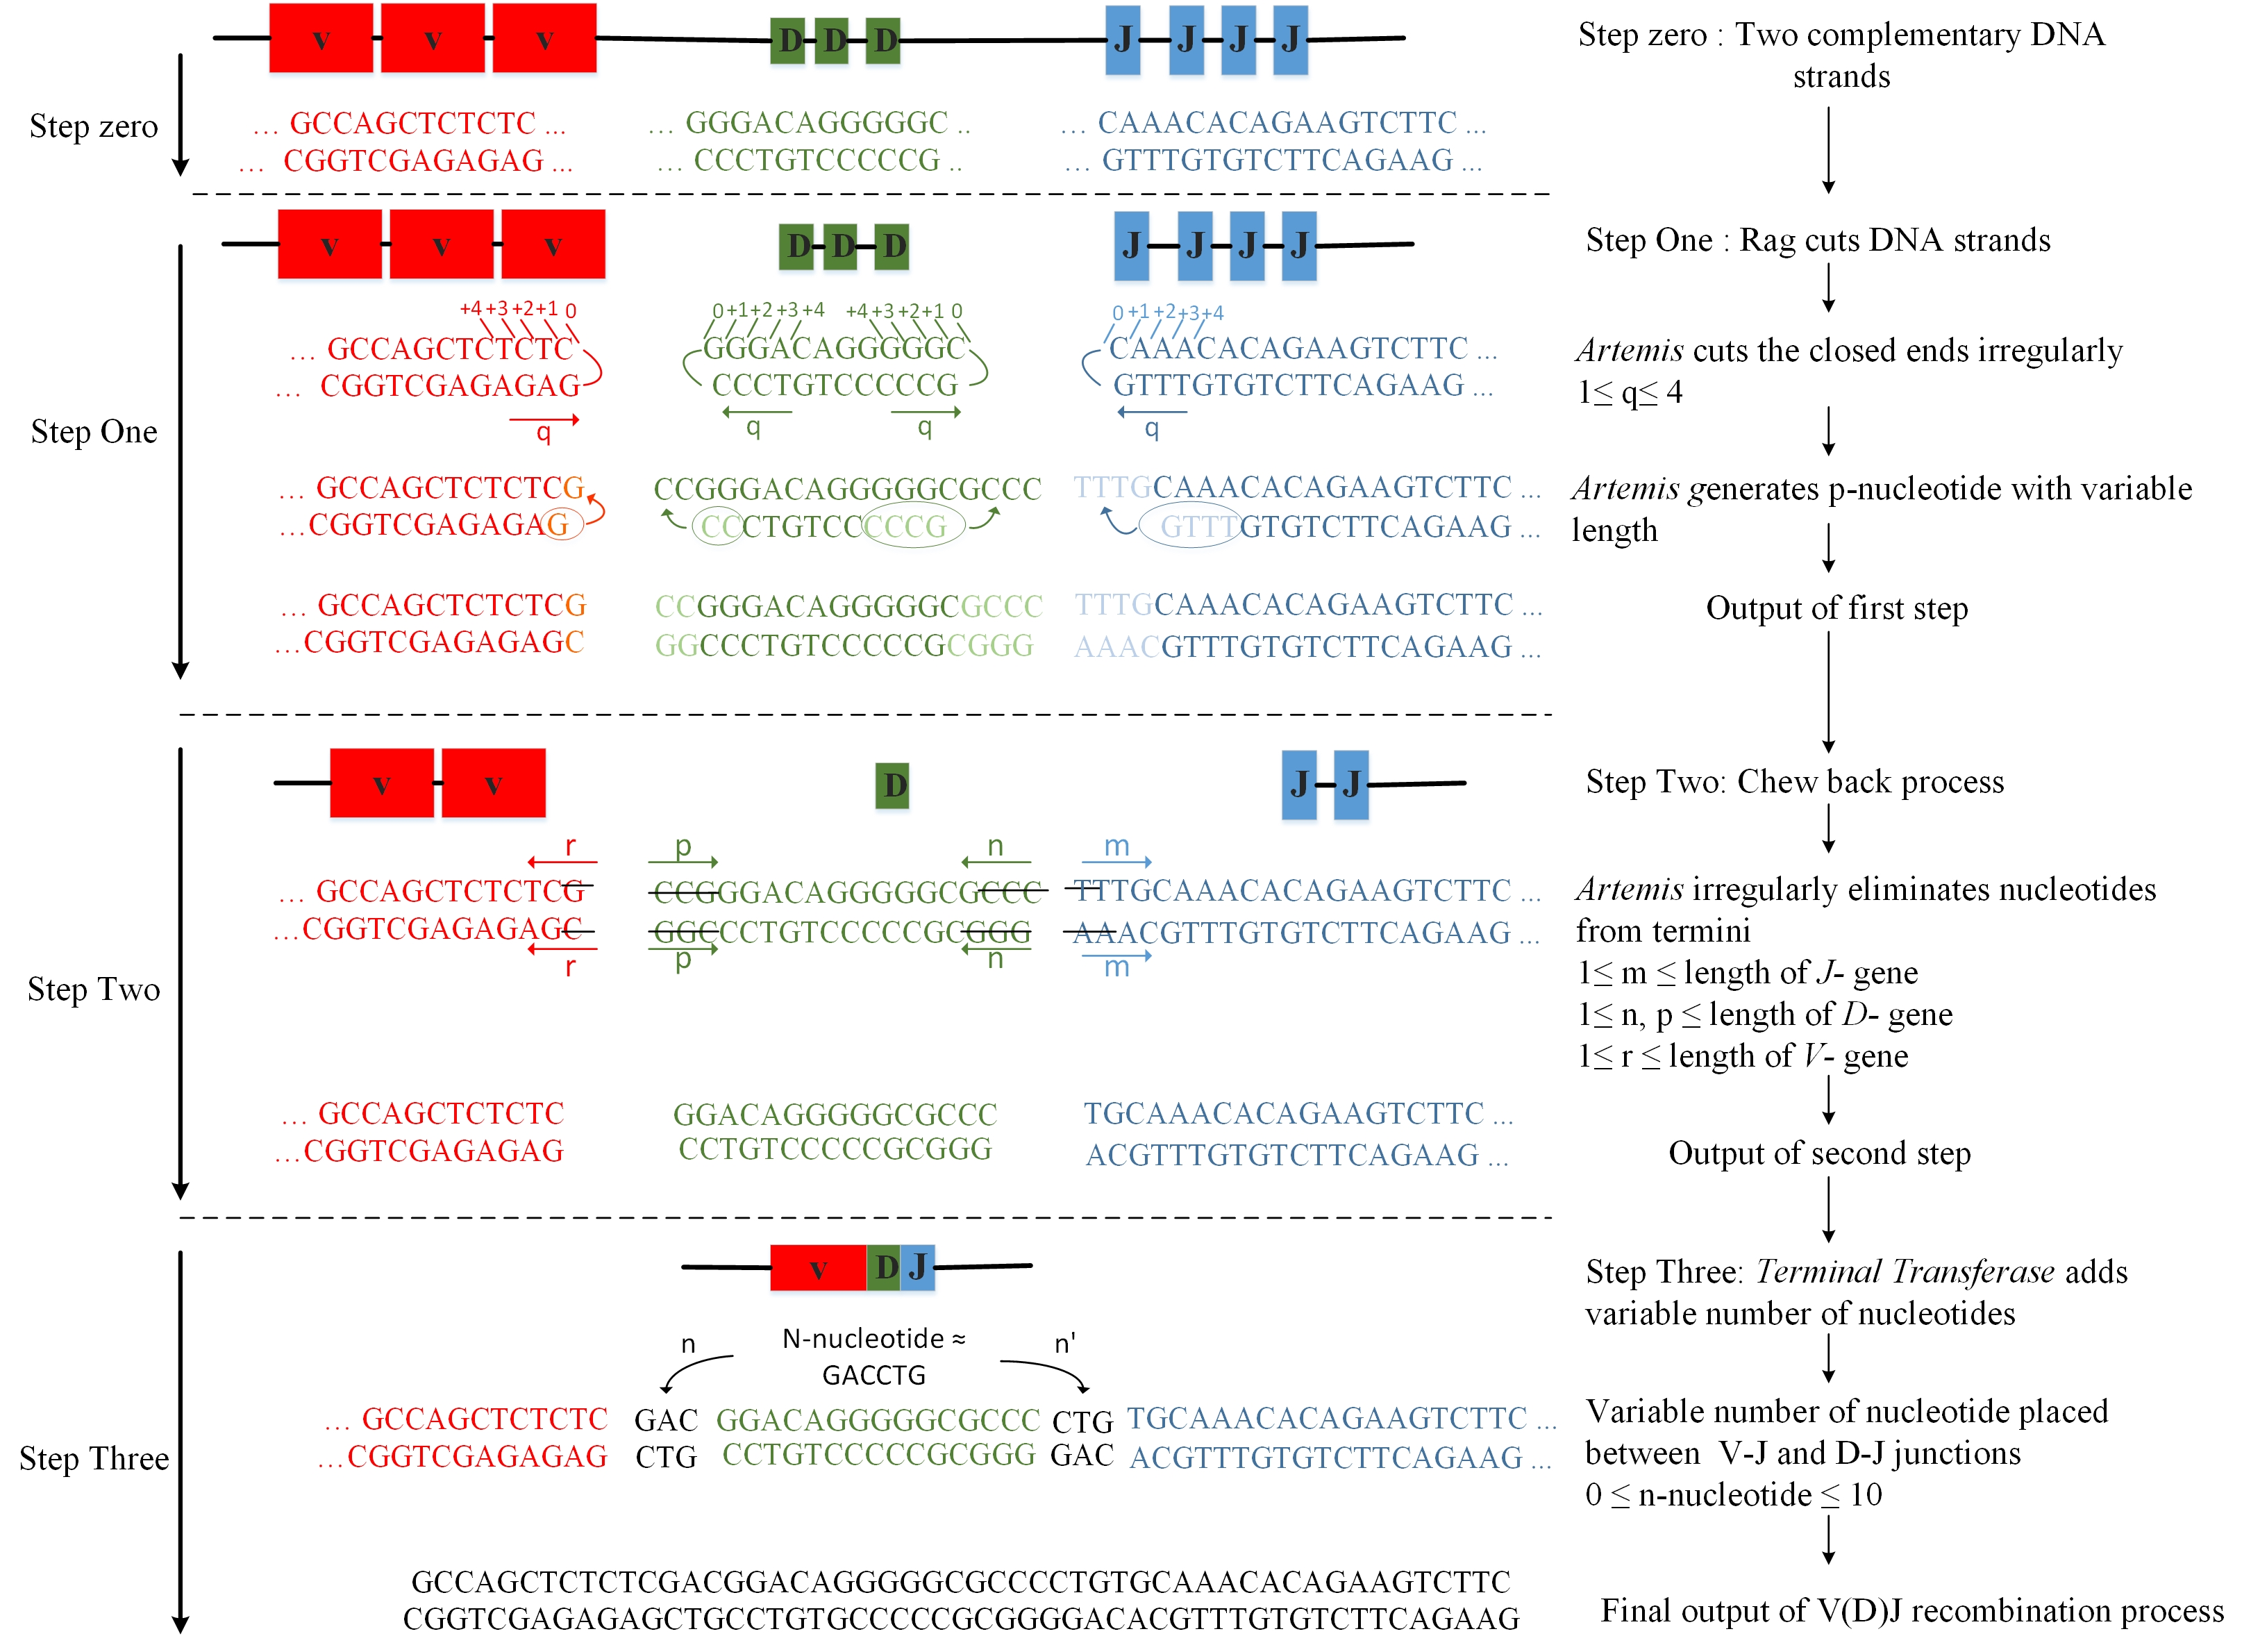
\includegraphics[clip,width=1\columnwidth]{Figure/V(D)J.jpg}
\caption{Brief view of the $V(D)J$ recombination process. The figure shows p-nucleotide formation with length one for $V-$ gene termini, two for left side of $D-$ gene termini, four for right side of $D-$ gene termini and four for $J-$ gene termini in step one. Example depicts elimination of one nucleotide on the $V-$ gene termini, three nucleotides on both side of the $D-$ gene and two nucleotides on $J-$ gene termini.}
\label{fig:VDJ}
\end{center}
\end{figure*} 
In the second step, both strands of the  $V$, $D$ and $J$ segments go through a process called chewback. Once more, the \emph{Artemis exonuclease} enzyme is involved in this chewback process, in which a variable number of nucleotide are eliminated from the $V$, $D$ and $J$ termini.  The chewback is applied from right to left on the $V$ segment, left to right on the $J$ segment, and from both directions on the $D$ segment. The amount of chewback ranges from one nucleotide to the length of that gene segment, which is the second contributor to the diversity.  
%Example shows elimination of three nucleotide on the right end and ? nucleotide on the left end of the $D-$ and two nucleotide from the $J-$ termini. 

In the third step, the \emph{Terminal Transferase (TDT)} enzyme catalyzes the addition of n-nucleotides between $V-D$  and $D-J$  gene pairs. We consider the size \emph{n} ranging between zero and ten. This range has been proven to regenerate $99.5\% $ of the sequences in our \emph{in vivo} data-set \cite{b2}. The \emph{in vivo} data set has been built based on the samples that were sequenced on the Roche FLX 454 platform at the UNC-Chapel Hill High Throughput Genome Sequencing Core. The \emph{in vivo} data set consists of 101,822 functional sequences. Finally, the DNA ligase \emph{IV} closes off the $V$ and $D$ termini to form $V-D$ junction, and $D$ and $J$ termini to form $D-J$ junction. Compared to the first two factors that contribute to the diversity, having n-nucleotide addition between $V-D$ and $D-J$ junctions enormously grow the combinational search space, and acts as the main contributor of the diversity.
%\vspace{-1.5 mm}
\subsection{Algorithmic Perspective}\label{subsec: algorithm}

We refer to the $V(D)J$ recombination as $VnDn'J$ recombination in this discussion about the algorithmic perspective. In this case, $V$, $D$, and $J$ indicate the unique sequences from each set of corresponding segments while `$n$' indicates the set of all possible nucleotide combinations. We refer the generated $VnDn'J$ sequences as the `\emph{in silico}' sequences. Thus, to generate the \emph{in silico} sequences, we need four inputs: $V$, $D$, $J$, and the n-nucleotide ($n$) sequences.

There are four bases: A, G, C, T, used to generate a n-nucleotide sequences. Thus, for n-nucleotide length $m$, there are $4^m$ unique combinations. In the recombination process, these n-nucleotide sequences can be attached on either side or on both sides of the $D$ sequence. To differentiate between the positions, we define the n-nucleotides as $n$ and $n'$. The $D$ sequence can cut the n-nucleotide at any position. Therefore, this complex junctional combination may lead to generation of an identical sequence through numerous ways. Our main purpose is to count the number of unique pathways that generate a given \emph{in vivo} sequence through the recombination process. Algorithm \ref{Algorithm:2} shows the pseudo code for the $VnDn'J$ recombination process with nested loops that iterate through each $V$, $D$, $J$ and $n$ sequence to form \emph{in silico} sequences. All single sequences are combined and stored in the variable \emph{Combination} through the nested loops. If a generated sequence is found in the current \emph{in vivo} set, we increment the counter value for that sequence. This process continues until the entire combinational search space is exhausted.    

\begin{algorithm}[t]
 \SetKwInOut{Input}{Input}\SetKwInOut{Output}{Output}\SetKwInOut{Init}{Initialization}
 \Input{$V$, $J$, $D$ and $n-nucleotide$ sequences}
 \Output{Number of times each unique \emph{in vivo} sequence is generated (Counter)}
\nl \For{$i = 0$ to number of $V$ sequences}{
\nl     \For{$j = 0$ to number of $J$ sequences}{
\nl     \For{$k = 0$ to number of $D$ sequences}{
\nl     \For{$m = 0$ to number of $n-nucleotide$ sequences}{
		\emph{Combination} = CombineString($V[i],n[m],D[k],n[m],J[j]$);
		
\nl		\For{$p = n-nucleotide_{lenght}$ to 0}{
		move ($N[m][p]$ $\to$ $T[n-nucleotide_{lenght}-p]$)		
		
\nl     \For{$n = 0$ to number of $in~vivo$ sequences}{
	 
		\If{$Combination == in vivo[n]$}{
			Counter[n]= Counter[n]+1;
		}
         }
      }
	}
  }
}
}
 \caption{Pseudo code for V(D)J Recombination Algorithm}
\label{Algorithm:2}
%vspace{-.5em}
\end{algorithm}

\subsection{Input data set}\label{subsec:input}
The input data sets consist of $V$, $D$, $J$ and \emph{in vivo} genes. In C57BL/6 mice, there are 20 basic $V \beta$ genes, 2 $D \beta$ genes and 12 basic $J \beta$ genes. However, all possible patterns such as chewback and palindromic forms for each of the functional $V$, $D$ and $J$ gene sequences need to participate in the recombination process for modeling the TCR repertoire as illustrated in  Fig. \ref{fig:VDJ}. 
For example, the first basic $V$ gene has a length of 14. For the $V$ gene, up to four genes can be appended to the right end of the $V$ gene from its mirror strand (step one, indicated as +4, +3, +2, +1), therefore the actual length of this gene can be up to 18. This would result with 18 different sequences based on the chewback process (step two). $D$ and $J$ gene data sets go through similar process as explained in Section \ref{subsec:Bio}, therefore each $V$, $D$ and $J$ gene data set consists of several forms of sequences with different lengths.  Each $V$, $D$, $J$, and \emph{in vivo} sequence is generated using four bases (A, G, T, and C). In C57BL/6 mice, the \emph{in vivo} data set involves 101,822 sequences, which are grouped based on the specific $VJ$ pair used to generate that sequence. There is no other recombination path for an \emph{in vivo} sequence other than the specific $VJ$ pair, which generates that specific sequence. This is a key feature that we can exploit to reduce a search space within the \emph{in vivo} data set and reduce the execution time. There are 240 such pairs since we have 20 basic $V$ genes and 12 basic $J$ genes in mice.
